\subsection{2020-01-15}
The following data structure represents a cash register. As it should be clear from the two accessor
functions, the first component represents the current item, while the second component is used to store
the price (not necessarily of the item: it could be used for the total). \\
\texttt{data CashRegister a = CashRegister { getReceipt :: (a, Float) } deriving (Show, Eq)} \\
\texttt{getCurrentItem = fst . getReceipt} \\
\texttt{getPrice = snd . getReceipt} \\
\begin{itemize}
    \item Make CashRegister an instance of Functor and Applicative
    \item Make CashRegister an instance of Monad.
\end{itemize}
Solution:
\begin{lstlisting}
    instance Functor CashRegister where
        fmap f cr = CashRegister (f $ getCurrentItem cr, getPrice cr)
    
    instance Applicative CashRegister where
        pure x = CashRegister (x, 0.0)
        CashRegister (f, pf) <*> CashRegister (x, px) = CashRegister (f x, pf + px)
    
    instance Monad CashRegister where
        CashRegister (oldItem, price) >>= f =
            let newReceipt = f oldItem
            in CashRegister (getCurrentItem newReceipt, price + (getPrice newReceipt))
\end{lstlisting}






\subsection{2019-09-03}
Consider the data structure Tril, which is a generic container consisting of three lists
\begin{itemize}
    \item 1) Give a data definition for Tril.
    \item 2) Define list2tril, a function which takes a list and 2 values x and y, say x < y, and builds a Tril, where the last component is the ending sublist of length x, and the middle component is the middle sublist of length y-x. Also, list2tril L x y = list2tril L y x. \\ E.g. list2tril [1,2,3,4,5,6] 1 3 should be a Tril with first component [1,2,3], second component [4,5], and third component [6].
    \item 3) Make Tril an instance of Functor and Foldable.
    \item 4) Make Tril an instance of Applicative, knowing that the concatenation of 2 Trils has first component which is the concatenation of the first two components of the first Tril, while the second component is the concatenation of the ending component of the first Tril and the beginning one of the second Tril (the third component should be clear at this point).
\end{itemize}
\begin{lstlisting}
    data Tril a = Tril [a] [a] [a] deriving (Show, Eq)

    instance Functor Tril where
        fmap f (Tril x y z) = Tril (fmap f x)(fmap f y)(fmap f z)

    instance Foldable Tril where
        foldr f i (Tril x y z) = foldr f (foldr f (foldr f i z) y) x
    
    (Tril x y z) +++ (Tril a b c) = Tril (x ++ y) (z ++ a) (b ++ c)

    trilconcat t = foldr (+++) (Tril [][][]) t
    trilcmap f t = trilconcat $ fmap f t

    instance Applicative Tril where
        pure x = Tril [x][][]
        x <*> y = trilcmap (\f -> fmap f y) x

    list2tril lst n1 n2 =   let (_,_,[x,y,z]) = foldr helper (n1, n2, [[]]) lst
                            in Tril x y z
        where
            helper el (0, m, next) = (-1, m-1, [el]:next)
            helper el (n, 0, next) = (n-1, -1, [el]:next)
            helper el (n, m, (x:xs)) = (n-1, m-1, (el:x):xs)
\end{lstlisting}




\subsection{2019-07-24}
Consider a non-deterministic finite state automaton (NFSA) and assume that its states are values of a type
State defined in some way. An NFSA is encoded in Haskell through three functions: \\
i) transition :: Char → State → [State], i.e. the transition function. \\
ii) end :: State → Bool, i.e. a functions stating if a state is an accepting state (True) or not. \\
ii) start :: [State], which contains the list of starting states. \\
\begin{itemize}
    \item 1) Define a data type suitable to encode the configuration of an NSFA.
    \item 2) Define the necessary functions (providing also all their types) that, given an automaton A (through transition, end, and start) and a string s, can be used to check if A accepts s or not.
\end{itemize}
\begin{lstlisting}
    data Config = Config String [State] deriving (Show, Eq)

    steps :: (Char -> State -> [State]) -> Config -> Bool
    steps trans (Config "" confs) = not . null $ filter end confs
    steps trans (Config (a:as) confs) = steps trans $ Config as (concatMap (trans a) confs)
\end{lstlisting}

\subsection{2019-06-28}
\begin{itemize}
    \item 1) Define a Tritree data structure, i.e. a tree where each node has at most 3 children, and every node contains a value.
    \item 2) Make Tritree an instance of Foldable and Functor.
    \item 3) Define a Tritree concatenation t1 +++ t2, where t2 is appended at the bottom-rightmost position of t1.
    \item 4) Make Tritree an instance of Applicative.
\end{itemize}
\begin{lstlisting}
    data Tritree a = Nil | Tritree a (Tritree a)(Tritree a)(Tritree a) deriving (Eq, Show)

    instance Functor Tritree where
        fmap f Nil = Nil
        fmap f (Tritree x t1 t2 t3) = Tritree (f x)(fmap f t1)(fmap f t2)(fmap f t3)

    instance Foldable Tritree where
        foldr f i Nil = i
        foldr f i (Tritree x t1 t2 t3) = f x $ foldr f (foldr f (foldr f i t3) t2) t1

    x +++ Nil = x
    Nil +++ x = x
    (Tritree x t1 t2 Nil) +++ t = (Tritree x t1 t2 t)
    (Tritree x t1 t2 t3) +++ t = (Tritree x t1 t2 (t3 +++ t))

    ttconcat t = foldr (+++) Nil t
    ttconcmap f t = ttconcat $ fmap f t

    instance Applicative Tritree where
        pure x = (Tritree x Nil Nil Nil)
        x <*> y = ttconcmap (\f -> fmap f y) x
\end{lstlisting}

\subsection{2019-02-08}
We want to define a data structure, called BFlist (Back/Forward list), to define lists that can either be “forward” (like usual list, from left to right), or “backward”, i.e. going from right to left. \\
We want to textually represent such lists with a plus or a minus before, to state their direction: e.g. +[1,2,3] is a forward list, -[1,2,3] is a backward list. \\
Concatenation (let us call it $<++>$) for BFlist has this behavior: if both lists have the same direction, the returned list is the usual concatenation. Otherwise, forward and backward elements of the two lists delete each other, without considering their stored values. \\
For instance: +[a,b,c] $<++>$ -[d,e] is +[c], and -[a,b,c] $<++>$ +[d,e] is -[c].
\begin{itemize}
    \item 1) Define a datatype for BFlist.
    \item 2) Make BFList an instance of Eq and Show, having the representation presented above.
    \item 3) Define $<++>$, i.e. concatenation for BFList.
    \item 4) Make BFList an instance of Functor.
    \item 5) Make BFList an instance of Foldable.
    \item 6) Make BFList an instance of Applicative.
\end{itemize}
\begin{lstlisting}
    data Dir = Fwd | Bwd deriving Eq
    data BFlist a = BFlist Dir [a] deriving Eq

    instance Show Dir where
        show Fwd = "+"
        show Bwd = "-"

    instance (Show a) => Show (BFlist a) where
        show (BFlist x y) = show x ++ show y
    instance Functor BFlist where
        fmap f (BFlist d x) = BFlist d (fmap f x)

    instance Foldable BFlist where
        foldr f i (BFlist d x) = foldr f i x
    
    (BFlist _ []) <++> x = x
    x <++> (BFlist _ []) = x
    (BFlist d1 x) <++> (BFlist d2 y) | d1 == d2 = BFlist d1 (x ++ y)
    (BFlist d1 (x:xs)) <++> (BFlist d2 (y:ys)) = (BFlist d1 xs) <++> (BFlist d2 ys)
    
    bflconcat (BFlist d v) = foldr (<++>) (BFlist d []) (BFlist d v)
    bflconcatmap f x = bflconcat $ fmap f x
    
    instance Applicative BFlist where
        pure x = BFlist Fwd [x]
        x <*> y = bflconcatmap (\f -> fmap f y) x
\end{lstlisting}

 
\subsection{2019-01-16}
We want to define a data structure, called Listree, to define structures working both as lists and as binary
trees, like in the next figure.
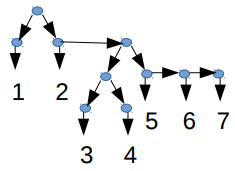
\includegraphics{haskell/2019-02-08.png}
\begin{itemize}
    \item 1) Define a datatype for Listree.
    \item 2) Write the example of the figure with the defined data structure.
    \item 3) Make Listree an instance of Functor.
    \item 4) Make Listree an instance of Foldable.
    \item 5) Make Listree an instance of Applicative.
\end{itemize}
\begin{lstlisting}
    data Listree a = Nil | Cons a (Listree a) | Branch (Listree a)(Listree a) deriving (Eq, Show)

    exfig = Branch (Cons 1 Nil) (Cons 2 (Branch (Branch (Cons 3 Nil) (Cons 4 Nil)) (Cons 5 (Cons 6 (Cons 7 Nil)))))

    instance Functor Listree where
        fmap f Nil = Nil
        fmap f (Cons x y) = Cons (f x) (fmap f y)
        fmap f (Branch x y) = Branch (fmap f x) (fmap f y)

    instance Foldable Listree where
        foldr f i Nil = i
        foldr f i (Cons x y) = f x (foldr f i y)
        foldr f i (Branch x y) = foldr f (foldr f i x) y

    x <++> Nil = x
    Nil <++> x = x
    (Cons x y) <++> z = (Cons x (y <++> z))
    (Branch x y) <++> z = (Branch x (y <++> z))

    ltconcat t = foldr (<++>) Nil t
    ltconcmap f t = ltconcat $ fmap f t

    instance Applicative Listree where
        pure x = (Cons x Nil)
        x <*> y = ltconcmap (\f -> fmap f y) x
\end{lstlisting}